%%%%% Document Setup %%%%%%%%

\documentclass[12pt, twocolumn]{revtex4}    % Font size (12pt) and column number (one or two).

\usepackage[a4paper, left=2.5cm, right=2.5cm, top=2.5cm, bottom=2.5cm]{geometry}  % Defines paper size and margin length

\usepackage{ragged2e}

\renewcommand{\baselinestretch}{1}     % Defines the line spacing

\usepackage{subcaption}
\usepackage[font=small, labelfont=bf, justification=justified, format=plain, singlelinecheck=off]{caption}\captionsetup{compatibility=false}

\usepackage{graphics,graphicx,epsfig,ulem}	% Makes sure all graphics works
\usepackage{amsmath} 						% Adds mathematical features for equations

\usepackage{etoolbox}                       % Customise date to preferred format
\makeatletter
\patchcmd{\frontmatter@RRAP@format}{(}{}{}{}
\patchcmd{\frontmatter@RRAP@format}{)}{}{}{}
\renewcommand\Dated@name{}
\makeatother

\usepackage{fancyhdr}

\pagestyle{fancy}                           % Insert header
\renewcommand{\headrulewidth}{0pt}
\lhead{\small Jacky Cao}                        
\rhead{\small The relation between stars and gas in distant galaxies}                

\def\thesection{\arabic{section}}
\def\thesubsection{\alph{subsection}}

\def\bibsection{\section*{References}}        % Position reference section correctly


%%%%% Document %%%%%
\begin{document}                     


\title{The relation between stars and gas in distant galaxies} 
\date{Submitted: \today{}}
\author{Jacky Cao}
\affiliation{\normalfont Level 4 Project, MPhys Physics\\ Supervisor: Dr.~Mark Swinbank\\ Department of Physics, Durham University}

\begin{abstract}              
 
 Observing any galaxy in the universe will yield the fact that it contains stars and also gas. The dynamics of both can be explored by observing galaxies and collecting spectroscopic data. 
 
Abstract abstract abstract abstract abstract abstract abstract abstract abstract abstract abstract abstract abstract abstract abstract abstract abstract abstract abstract abstract abstract abstract abstract abstract abstract abstract abstract abstract abstract abstract abstract abstract abstract abstract abstract abstract abstract abstract abstract abstract abstract abstract abstract abstract abstract abstract abstract abstract abstract abstract abstract abstract abstract abstract 

\end{abstract}


\maketitle
%\thispagestyle{plain} % produces page number for front page

\tableofcontents
%\let\toc@pre\relax
%\let\toc@post\relax

\newpage

\section{Introduction} 

Amongst the different types of cosmic structure within our universe, galaxies can be seen as the island powerhouses of industry and activity. Containing countless stars, gas, dust, and dark matter \cite{carroll_astro}, it would be difficult not to express the statement that the motions of these objects must be linked in some galactic relationship. 

By utilising the most powerful tool in astronomy, observation, galaxies, their structure and the motions of the objects within them can be studied to a great depth. As an example, if we took optical measurements of the stellar population, we could use that information to estimate the potential age of the galaxy. We know that redder stars are older and bluer stars represent a younger set of objects \cite{carroll_astro}. Or if we wanted to know about the material composition or even the distance to a certain galaxy, we could split the collected light in a spectrograph to produce a spectrum. Values of redshift and the content of a galaxy can be obtained by looking at the absorption and emission lines within a galactic spectrum \cite{carroll_astro}.

Gathering and processing this optical and spectroscopic information allows us to build a broad picture of the internal workings of a galaxy. Then with further analysis we can begin to comprehend the intricate relationships contained within these individual islands. 

To begin with we must consider a general picture of galaxies, after which we will be able to appreciate and explore the more complex ideas [???].

\subsection{Galactic classification}

As we stated previously, a galaxy can be quite broadly defined as a collection of gas, dust, stars and dark matter. But if we were to observe a large enough sample then we would begin to see that the galaxies can be grouped and classified together.

This categorisation is called the \textit{Hubble Sequence} or the \textit{Hubble Tuning Fork} \cite{carroll_astro}. From Figure \ref{fig:hubble_tuning_fork} we can see that galaxies can be divided into ellipticals, spirals and irregulars. With ellipticals along the horizontal handle, the two prongs containing normal and barred spirals, and finally irregulars as the third category. The sequence itself does not show the evolution of the galaxies, rather it provides a way to view the different morphologies of galaxies on one plot.

\begin{center}
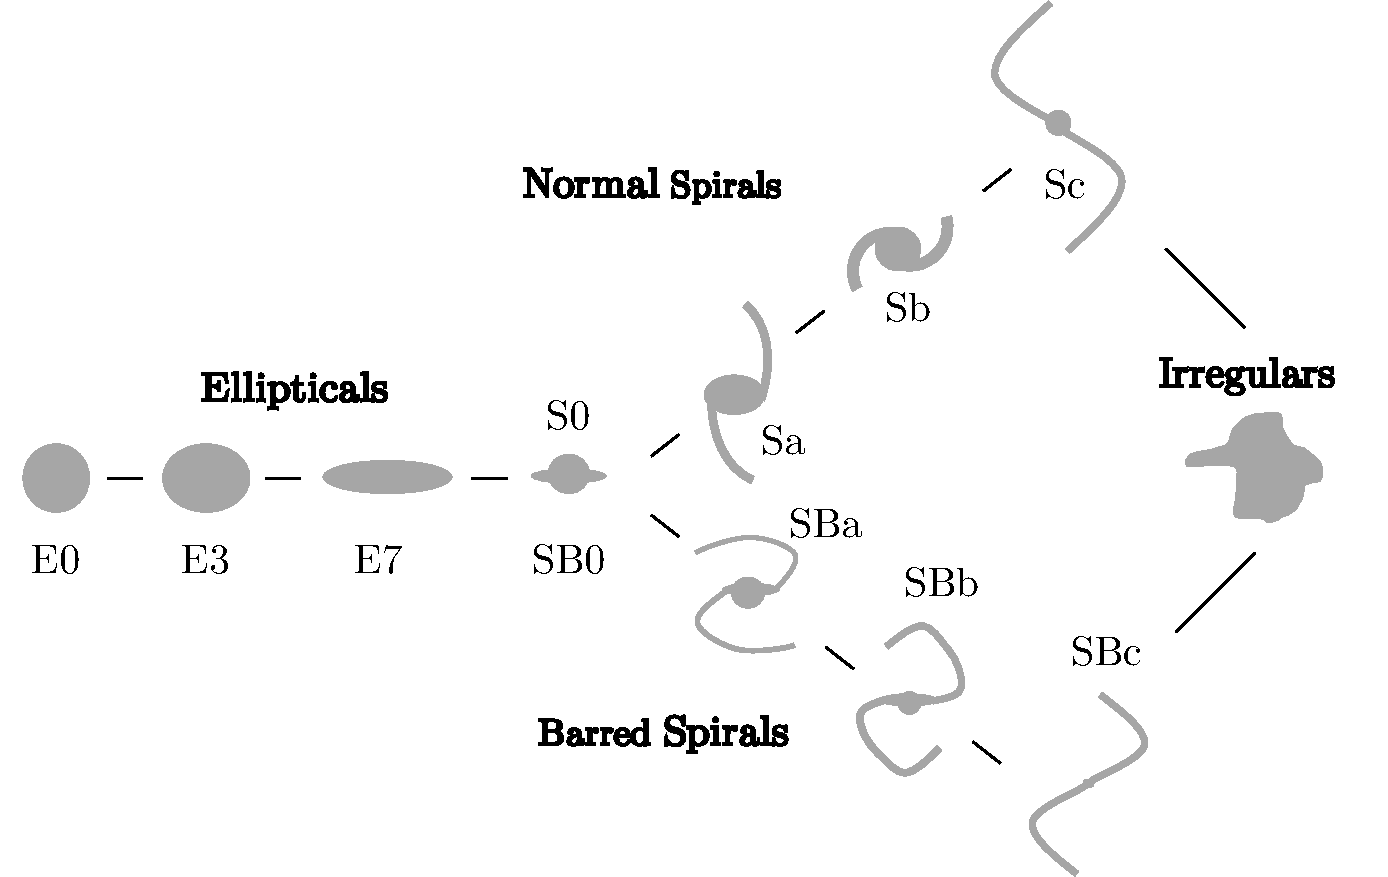
\includegraphics[width=1.0\linewidth]{introduction/hubble_tuning_fork}
\captionof{figure}[Hubble Tuning Fork]{The Hubble Sequence, containing three general groups of ellipticals, spirals, and irregular galaxies. The diagram does not show the evolution of galaxies but their classification. \\ (\textit{This diagram has been adapted from An Introduction to Modern Astrophysics} \cite{carroll_astro}.)}
\label{fig:hubble_tuning_fork}
\end{center}

We must ask ourselves then what each grouping represents in relation to the make-up of the galaxy. Alongside the classification through shape and general appeareance we can also explore the component composition of the three general types of galaxies. Take ellipticals to begin with, we can see from the Hubble Tuning Fork that they are composed of a spherical-like distribution of matter. The stellar objects within elliptical galaxies are mainly older red stars. 

- from describing the composition of the stars and 'old elliptical stars' we can then go on to discuss the star forming rates and initial mass function

Take ellipticals, the distribution of stellar objects within these galaxies are dominated by mainly redder old stars. [???] These types of galaxies coalesce into a spherical-like collection. Comparatively, spiral galaxies are composed of a central bulge which has old stars and a surrounding disk or protruding arms which contain younger stellar objects \cite{carroll_astro}. Irregular galaxies have no noticeable symmetry and no obvious central nucleus, so they do not fall into either of the other two categories.

- I should expand on how galaxies can actually be identified from one another
- currently my theory for them is a bit meh, there's not much substance between them
- there should just be more expalanation

By knowing these general characteristics, as we continually to improve our observational instruments we can then view deeper into the Universe's past. This means the galactic objects are becoming more and more younger, this is a powerful way for us to build a picture of the evolutionary nature of galaxies and their structure. 

\subsection{Galactic and stellar formation}

- discuss galaxies generally, from the hubble tuning fork to how we an class the individual three groups
- then we can move onto the formation of galaxies, discussing stellar formation rates and the initial mass function
- we want to build up a short but complete picture of what galaxies are 

We introduced the concept that through optical measurements of the stars 

What do I want to say with this? I want to introduce galaxies, the different types of galaxies, how they form, how they can be confused with other types of structure. 

\subsection{Data} 

askjdnaksld

\subsubsection{HUDF and MUSE}

To obtain spectroscopic information on the Hubble UDF objects, the Multi-Unit Spectroscopic Explorer or MUSE was employed. This instrument is 

what is MUSE, where it is on the VLT, problems, limitations of MUSE - why it is useful...etc

\onecolumngrid

\begin{figure}
  \begin{subfigure}[b]{0.4\textwidth}
    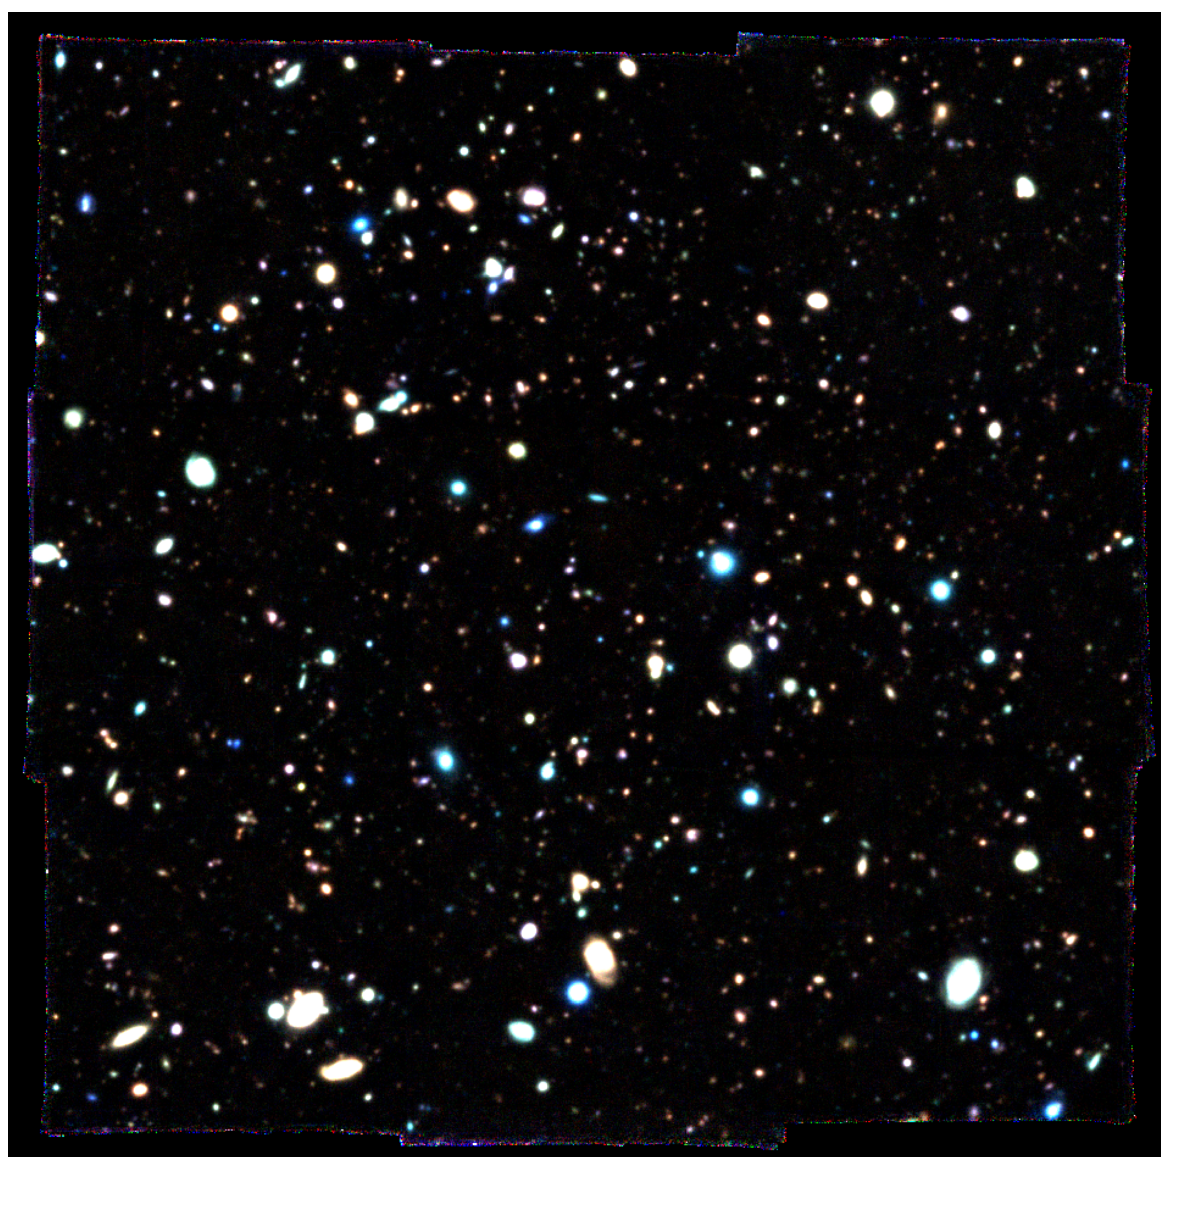
\includegraphics[width=\textwidth]{introduction/muse_colour_image}
    \captionsetup{justification=justified}    
    \caption{MUSE HUDF}               
    \label{fig:muse_colour_image}
  \end{subfigure}
  %
  \begin{subfigure}[b]{0.4\textwidth}
    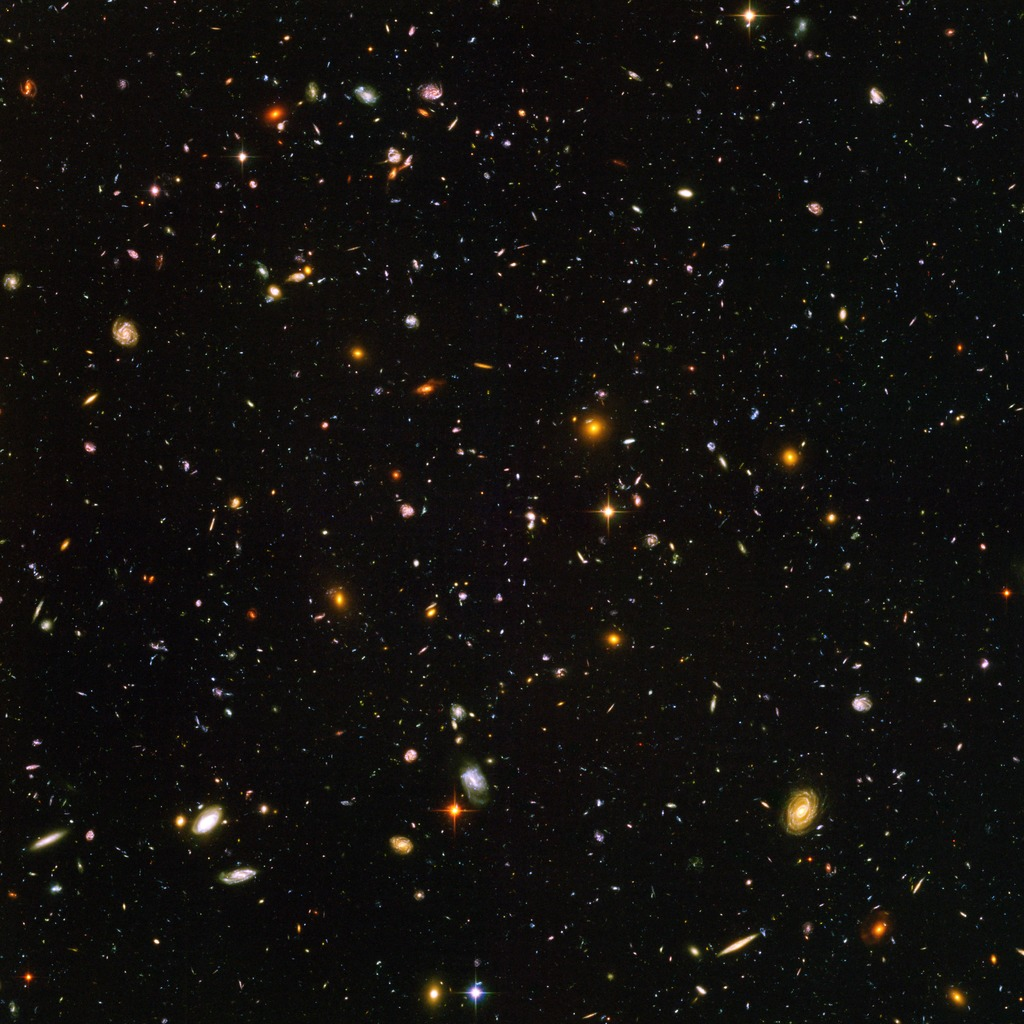
\includegraphics[width=\textwidth]{introduction/hubble_ultra_deep_field}
    \captionsetup{justification=justified}    
    \caption{HST HUDF}
    \label{fig:hubble_ultra_deep_field}
  \end{subfigure}
  \caption[Hubble Ultra Deep Field]{(a) A colour image created from the MUSE spectroscopic data of the HUDF. The wavelength range was split into three equal regions and then collapsed to create three bands (R, G, B). A final colour image was produced by combining these separate frames together. (b) The optical HUDF as captured by the Advanced Camera for Surveys instrument on the Hubble Space Telescope \cite{hudf_image}. }
\end{figure}

\twocolumngrid

asdasd

\section{Analysis} 

sfsadf

\subsection{Cube extraction}

asdasd

\onecolumngrid

\begin{figure}
  \begin{subfigure}[b]{0.495\textwidth}
    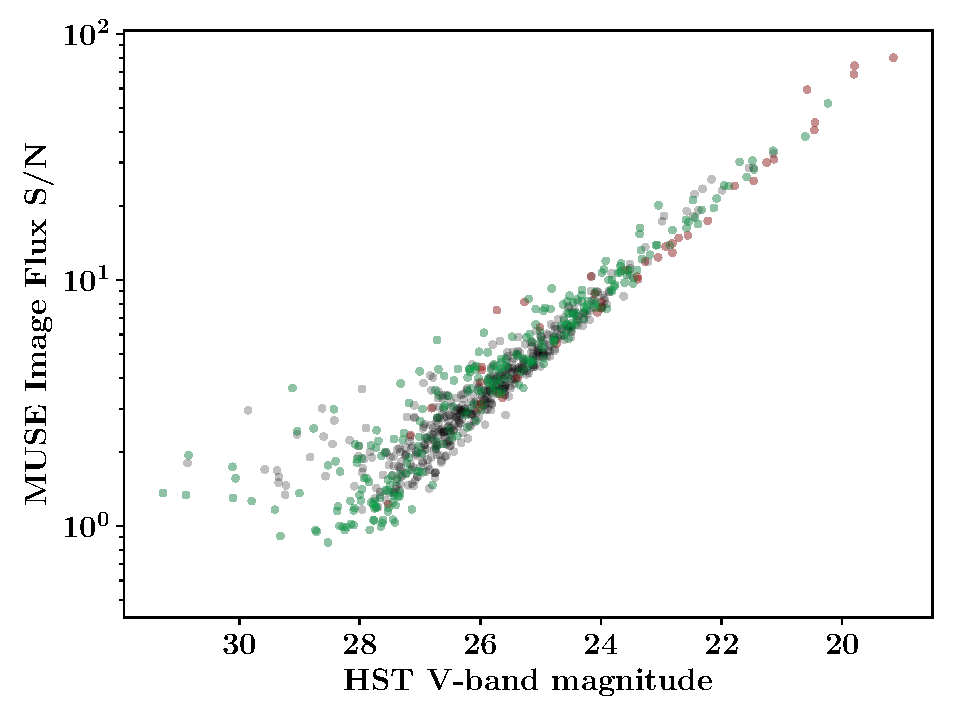
\includegraphics[width=\textwidth]{data/image_sn_vs_vband}
    \captionsetup{justification=justified}
    \caption{Image S/N vs. V-band}
    \label{fig:image_sn_vband}
  \end{subfigure}
  %
  \begin{subfigure}[b]{0.495\textwidth}
    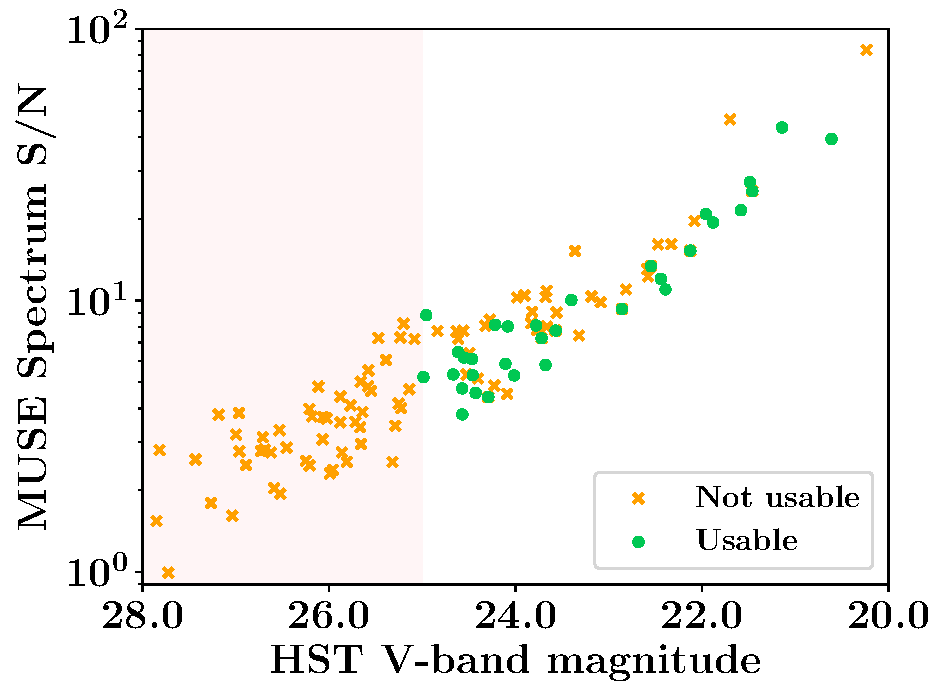
\includegraphics[width=\textwidth]{data/sn_vs_vband}
    \captionsetup{justification=justified}    
    \caption{Spectroscopic S/N vs. V-band}
    \label{fig:spec_sn_vband}
  \end{subfigure}
  \caption[HUDF Objects]{---}
\end{figure}

\twocolumngrid

sdfsadf

\subsection{pPXF} 

-

\section{Discussion} 

-

\section{Conclusions}
 
In conclusion, through extensive data and statistical analysis it can be said that the dynamics of stars and gas in galaxies are ... (?) 

\begin{acknowledgments}
The author would like to thank Dr.~M.~Swinbank and Dr.~A.~Tiley for their continual help and support throughout the project period, without which, the project would have been experimentally grounded.
\end{acknowledgments}

\bibliographystyle{unsrt}
\bibliography{stars_gas_dynamics}

\end{document}